\documentclass[10pt,a4paper,oneside]{beamer}

\usetheme{Boadilla}

\usepackage[utf8]{inputenc}
\usepackage[german]{babel}
\usepackage{amsmath}
\usepackage{amsfonts}
\usepackage{amssymb}
\usepackage{hyperref}
\usepackage{biblatex}
\usepackage{wrapfig}
\addbibresource{bib}

\title{Inertialnavigation bei autonomen Flugkörpern}
\author{
	Fabian Ulbricht \and
	Paul Walger 
}

\begin{document}

%% Start
\frame{
	\titlepage
}

\frame {
	\frametitle{Inhaltsverzeichnis}
	\tableofcontents
}

\begin{frame}
  \section{Einleitung}
  \frametitle{Einleitung}
  
  Positionsbestimmung war und ist ein Problem das nicht einfach zu lösen ist.
  Es wurde auf vielfältige Weisen versucht zu lösen, vom Kompass und Sextant bis zu GPS.\\
  Wir werden uns auf die Inertialnavigation begrenzen. 
\end{frame}


\begin{frame}
	\section{Trägheitsnavigation}
	\frametitle{Trägheitsnavigation}
	In sich abgeschlossen Navigationstechnik, 
	welche die Position und Orientierung eines Objektes relativ zu einem Start-punkt, orientierung und geschwindigkeit bestimmt.
	
	Besteht aus:
	\begin{enumerate}
		\item Computer
		\item Accelerometer
		\item Gyroskop
	\end{enumerate}
	
	2 Hauptgruppen von Konfigurationen \cite{Wood07}
	\begin{enumerate}
		\item Stable Platform Systems
		\item Strapdown Systems
	\end{enumerate}
\end{frame}

\begin{frame}
	Stable Platform Systems
	\resizebox{\textwidth}{0.4\textheight} {
	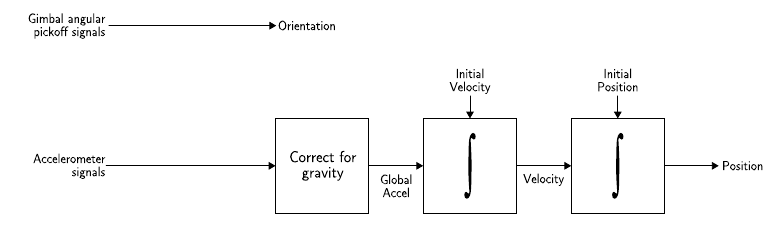
\includegraphics[scale=1]{images/stable_platform.png} 
	}
	\bigskip
	Strapdown Systems
	\resizebox{\textwidth}{0.4\textheight} {
		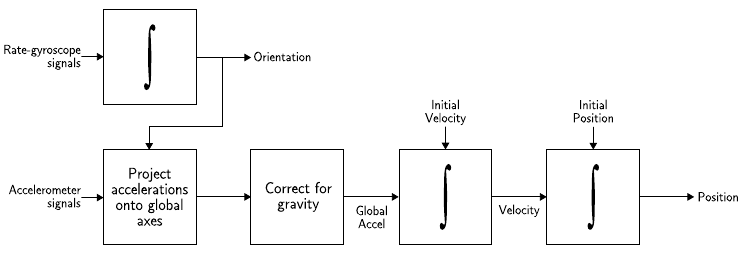
\includegraphics[scale=1]{images/strapdown.png} 
	}

\end{frame}

\begin{frame}
	\section{Autonome Flugköper}
	\frametitle{Autonome Flugköper = Cruise Missile}
	Beschreibung: \cite{GS04}
	
	\begin{itemize}
		\item Dispensable
		\item Pilotless
		\item Self-Guided
		\item Continously Powerd
		\item Air-Breathing
	\end{itemize}
	
	Anforderungen an die INS:\\
	\begin{itemize}
		\item 20 Hz Update
		\item Mehre Stunden Flugzeit
		\item Short-Term Accuracy
		\item Bestimmung von missile position, velocity, attitude, and altitude
	\end{itemize}
	
\end{frame}

\begin{frame}
	\section{Sensoren}
	\frametitle{Sensoren}
	Zwei Gruppen von Sensoren:
	\begin{itemize}
		\item Geschwindikeit = Accelorometer
		\item Orientierung = Gyroscope
	\end{itemize}
	
	Hohe Anforderungen von Genauigkeit wegen der Akkumulierung von Fehlern.\\
	Die Größe muss auch minimal sein, da die Flugkörper klein sind.

\end{frame}

\begin{frame}
  \subsection{Acceloremeter}
  \frametitle{Acceloremeter (Beschleunigungssensoren)}
  
  Anwendung:
  \begin{itemize}
    \item Messung von (linearen) Beschleunigungen
  	\item Sensorik in digitalen Kameras
  	\item Positionsbestimmung
  \end{itemize}
\end{frame}

\begin{frame}
  \frametitle{MEMS Acceloremeter}
  
  \begin{definition}[MEMS]
  = Microelectromechanical systems \\
  Sehr kleine mechanische Geräte angetrieben durch Elektrizität.
  \end{definition}
  \medskip 
  2 Typen von Acceloremtern:
  \begin{itemize}
    \item Piezoelectric accelerometer
  	\item Surface micromachined capacitive
  \end{itemize}
\end{frame}

\begin{frame}
  \frametitle{Piezoelectric accelerometer}
  Wirkungsweise: Die bei Beschleunigung Änderung der einwirkenden Kraft wird mittels des Piezoelektrischen Effekts gemessen.
  Konstante Beschleunigungen können nicht gemessen werden.
    \bigskip
    \begin{definition}[Piezoelektrizität]
		Beschreibt das Auftreten einer elektrischen Spannung an Festkörpern, wenn sie elastisch verformt werden.
	\end{definition}
\end{frame}

\begin{frame}
	\frametitle{Capacitive acceloremters}
	\begin{block}{Funktionsweise}
		Messung von Kapazitätsänderungen.
	\end{block}

    \bigskip
    
	Vorteile
 	\begin{itemize}
 		\item Herstellung mit herkömmlicher MEMS Technologie möglich
 		\item Hervorragende Sensibilität
		\item Unabhängig von Außentemperatur
 	\end{itemize}
\end{frame}

\begin{frame}
	\frametitle{Kapazität}
	Die Kapazität von 2 parallen Platten ist \cite{AM08}
	\begin{equation}
		C_{0} = \epsilon_{0} \epsilon_{r} \frac{A}{d} = \epsilon_{A} \frac{1}{d}
	\end{equation}
	
	wobei $\epsilon_{A} = \epsilon_{0} \epsilon_{r} A$ und A die Fläche der Elektroden, d die Distanz zwischen ihnen und die $\epsilon_{r}$ die Perimitivität von dem Material dass die beiden trennt.

\end{frame}

\begin{frame}
	\frametitle{Kapazität 3}

\begin{wrapfigure}{l}{0.4\textwidth}

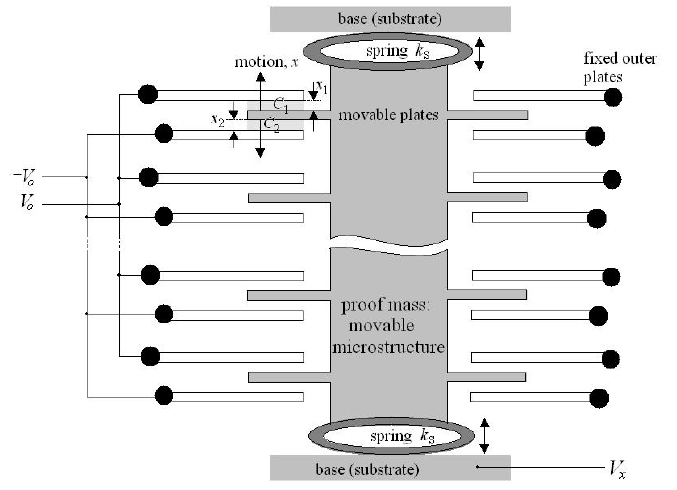
\includegraphics[width=0.4\textwidth]{images/acceleromter_structure.png}

\end{wrapfigure}

Die Kapazitäten $C_{1}$ und $C_{2}$ zwischen der beweglichen Platte und den äußeren Stationären Platten sind abhängig von den Verschiebung $x_{1}$ und $x_{2}$.
	\begin{equation}
		C_{1} = \epsilon_{A} \frac{1}{x_{1}} 
			  = \epsilon_{A} \frac{1}{d+x} 
			  = C_{0} - \Delta C
	\end{equation}
	
	\begin{equation}
		C_{2} = \epsilon_{A} \frac{1}{x_{2}} 
		      = \epsilon_{A} \frac{1}{d-x} 
		      = C_{0} + \Delta C
	\end{equation}
	
\end{frame}

\begin{frame}
	\frametitle{Kapazität 4}
	
	Wenn die Beschleunigung null ist, dann sind die Kapazitäten $C_{1}$ und $C_{2}$ gleich.
	Wenn aber $x_{1} \neq x_{2}$ also $x \neq 0$ dann gilt:
	\begin{equation}
		C_{1} - C_{2} = 2 \Delta C = 2 \epsilon_{A} \frac{x}{d^{2}-x^{2}}
	\end{equation}
	
	Wenn wir nun $\Delta C$ messen, dann könne wir die Verschiebung $x$ messen indem wir die nichtlineare algebraische Gleichung lösen.
	
	\begin{equation}
		\Delta C x^{2} + \epsilon_{A} x + \Delta C d^{2} = 0
	\end{equation}
	
	Für kleine Verschiebungen ist der Term $\Delta C x^{2}$ verschwindend klein. Es gilt also
	\begin{equation}
		x \approx \frac{d^{2}}{\epsilon_{A}} \Delta C = d \frac{\Delta C}{C_{0}}
	\end{equation}
	Wir können also sagen, dass die Verschiebung annähernd proportional ist zur Kapazitätsdifferenz $\Delta C$
\end{frame}

\begin{frame}
  \subsection{Gyroskop}
  \frametitle{Gyroskop (Rotationssensoren)}
  
  \begin{block}{Was ist ein Gyroskop}
  	Ein Gerät zur Messung oder Erhaltung der Orientierung, basierend auf dem Prinzip des Drehimpulses.
  \end{block}
  
  \bigskip
  
  Typen von Gyroskopen
  \begin{enumerate}
  	\item Mechanisch
  	\item Optisch 
  	\item MEMS
  \end{enumerate}
\end{frame}

\begin{frame}
	\frametitle{Mechanische Gyroskope}
	%% http://www.ipgp.fr/~lucas/Contrib/animbeamer.html
	\begin{wrapfigure}{l}{0.4\textwidth}
	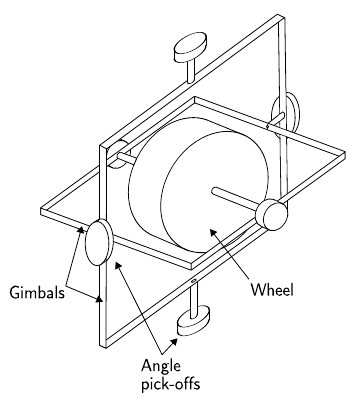
\includegraphics[width=0.4\textwidth]{images/mechanical_gyroscope.png} 
	\end{wrapfigure}
	
	Bestehen aus einem spinning wheel und zwei Gimbals, welche es eine Rotation in 3-Achsen erlaubt. \\
	Ein Mechanische Gyroskope misst die Orientierung direkt, 
	während die meisten moderne Gryoskope die Winkelgeschwindigkeit messen.
	
	Nachteile:
	\begin{enumerate}
	  	\item Bewegliche Teile
	  	\item Reibung
	  	\item Ein paar Minuten Aufwärmzeit benötigt
	  \end{enumerate}

\end{frame}

\begin{frame}
	\frametitle{Optische Gyroskope}
	\begin{wrapfigure}{l}{0.4\textwidth}
	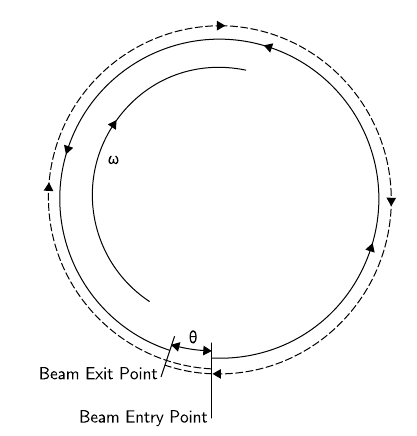
\includegraphics[width=0.4\textwidth]{images/fog.png} 
	\end{wrapfigure}
	
	Insbesondere Faserkreisel (Fibro Optic Gyroscope = FOG). \\
	Besteht aus einer langen Spule von Glasfasern. Es werden zwei Lichtimpluse in entgegengesetze Richtung abgefeuert. Wenn das System rotiert, erfährt der eine Lichtimplus eine längere Laufzeit.\\
	Gemessen wird über die Interferenz von den beiden Lichimplusen.

\end{frame}

% Ich denke wir stellen zuerst allgemein den Kalman-Filter dar.

\begin{frame}
  \section{Kalman-Filter}
  \frametitle{Kalman-Filter}
\end{frame}

\begin{frame}
  \frametitle{Diskreter Kalman-Filter}
  
\end{frame}

\begin{frame}
  \section{Bewegunsgleichungen}
  \frametitle{Modelierung eines Systems}
\end{frame}

\begin{frame}
  \section{Kalman-Filter für UAV}
  \frametitle{Kalman-Filter für UAV}
\end{frame}

\begin{frame}
  \section{Literatur}
  \frametitle{Literatur}
\printbibliography

\end{frame}


\end{document}
